\chapter{Risultati}
\label{chap:Results}

In questo capitolo vengono illustrati i risultati ottenuti. Per quanto riguarda il miglioramento
della gestione dei progetti, vengono presentate le soluzioni proposte e accettate dalla direzione,
mirate a rendere il lavoro più efficiente. Per quanto riguarda lo sviluppo dell’applicativo \ac{PAM},
invece, si riporta l’interfaccia principale realizzata, fornendo una visione chiara del contributo
pratico apportato.

\section{Gestione Progetti}
Sulla base delle proposte illustrate nel Capitolo \ref{chap:pm}, la direzione e il responsabile dei
project manager hanno concordato di rendere immediatamente obbligatorie alcune pratiche in ogni fase
del ciclo di vita di un progetto, applicandole sin da subito ai nuovi progetti.
La decisione è stata accolta positivamente da tutti i dipendenti, con la volontà comune di allinearsi per migliorare
la qualità del lavoro, riconoscendo l’utilità e l’applicabilità immediata delle soluzioni individuate.
Le azioni descritte di seguito, suddivise per ciascuna fase progettuale, rappresentano quelle maggiormente adattate
alle esigenze aziendali. Partendo dalle proposte iniziali, sono state perfezionate attraverso un confronto diretto
con la direzione e i project manager, garantendone una migliore integrazione nel contesto operativo.

    \subsection{Idea, Design, Economics}
    Nella fase iniziale, quando il progetto non è ancora confermato e l'obiettivo è valutare il potenziale interesse
    del cliente, verranno svolte una serie di \textbf{riunioni esplorative con il committente}.
    Dal momento che in azineda non è presente una figura commerciale, durante gli incontri sarà il CEO ad occuparsi
    di convincere il cliente ad acquistare un nuovo sistema. Le conversazioni
    possono includere la visione di alcuni mockup o presentazioni per dare un'idea preliminare delle soluzioni realizzabili.

    Quando un cliente decide di avviare un nuovo progetto, viene assegnato un project manager di riferimento.
    Per garantire un \textbf{allineamento} iniziale efficace, si svolge un breve incontro \textbf{tra il CEO e il project manager},
    durante il quale il primo fornisce il contesto del progetto in modo informale.
    Questo confronto permette di chiarire gli obiettivi e definire una base solida per la gestione complessiva.

    Successivamente si passa a \textbf{incontri più strutturati con il cliente} per approfondire le idee, definire gli obiettivi
    e individuare le aree di maggiore interesse. A queste riunioni di approfondimento partecipano sia il CEO che il project
    manager, utilizzando mockup più dettagliati per affinare le specifiche e garantire una visione chiara del progetto.

    Man mano che si svolgono le riunioni, le informazioni raccolte vengono inserite e aggiornate nei documenti Confluence,
    con particolare attenzione ai \textbf{requisiti funzionali e non funzionali}. Questa attività viene svolta
    congiuntamente dal CEO e dal project manager, garantendo una documentazione chiara e sempre aggiornata.

    \subsection{Progetto Software}
    \subsubsection{Avvio}

    Subito dopo aver concordato con il cliente le specifiche del progetto, viene individuata la persona responsabile
    della gestione operativa, il \textbf{team leader}, il quale ha il compito di coordinare le attività tecniche di sviluppo.

    Tutti i \textbf{documenti} prodotti nelle fasi precedenti vengono \textbf{condivisi} al team leader, permettendogli di
    acquisire una visione chiara del progetto prima dell’inizio delle attività operative.

    Dopodiché, si organizza una \textbf{riunione di allineamento interna} rapida (massimo tenta minuti) tra il team leader,
    project manager e CEO, così da chiarire eventuali dubbi emersi dopo l’analisi della documentazione e definire gli aspetti principali del progetto.

    In incontri successivi, il project manager e il team leader \textbf{analizzano i rischi} suddividendoli in diverse categorie: tecnici,
    di project management, organizzativi ed esterni. Per quelli legati alla sicurezza informatica, si utilizza il modello STRIDE illustrato precedentemente.
    L’impatto e la probabilità di ogni rischio vengono classificati attraverso la matrice di rischio, suddivisa nei tre livelli: basso, medio e alto.

    Per quanto riguarda la \textbf{definizione delle risorse umane necessarie}, si identificano sin da subito le figure professionali richieste
    per lo sviluppo del progetto. Ad esempio, se tutte le \ac{PBC} necessarie sono
    già disponibili, potrebbero servire solo sviluppatori frontend per implementare l’interfaccia grafica, senza necessità di risorse backend.
    
    \subsubsection{Pianificazione}
    La suddivisione del lavoro in attività e sottoattività a livello logico deve essere organizzata in una \textbf{\ac{WBS}} ad albero,
    utilizzando una lavagna condivisa su \textbf{Miro}. Questo permette una visualizzazione chiara della struttura del progetto e
    facilita la collaborazione tra i membri del team.

    Per la \textbf{pianificazione} ad alto livello di progetto sarà obbligatorio creare un \textbf{Gantt} con l’utilizzo di GanttPRO.
    Questo strumento consente di definire una pianificazione temporale dettagliata, individuando le dipendenze tra le attività.
    Il piano deve essere condiviso e aggiornato con il cliente.

    Per garantire una gestione ordinata ed efficace del progetto, è fondamentale attenersi alle linee guida definite per
    la \textbf{pianificazione e progettazione su Jira}. Epic, task e subtask devono essere strutturati in modo coerente,
    partendo dalla \ac{WBS} e rispettando la gerarchia indicata. Il project manager sarà responsabile della definizione di epic e task,
    mentre il team leader si occuperà di dettagliare le attività tecniche operative attraverso la creazione dei subtask.

    \subsubsection{Esecuzione}
    Per definire standard aziendali condivisi, i quali servono a garantire coerenza e qualità nel lavoro di tutti, sarà necessario
    svolgere una \textbf{riunione sulle linee guida per gli sviluppatori} il prima possibile, nella quale si parlerà di:
    \begin{itemize}
        \item \textbf{convenzioni tecniche}, tra cui la nomenclatura di commit, branch e altre pratiche di versione del codice;
        \item \textbf{documentazione del codice}, con particolare attenzione alla spiegazione delle logiche complesse adottate;
        \item aggiornamento costante della \textbf{documentazione di progetto}, includendo qualsiasi modifica significativa,
        ad esempio il cambiamento della struttura dati di una \ac{PBC}.
    \end{itemize}

    Alla fine di ogni giornata lavorativa, è essenziale \textbf{aggiornare i subtask} su cui si è lavorato. Oltre a
    registrare le ore impiegate, ciascun dipendente deve modificare lo stato di avanzamento dei compiti svolti e aggiungere
    un riepilogo delle attività svolte nella sezione relativa ai commenti, oltre a eventuali difficoltà riscontrate.
    
    Tutte le \textbf{scadenze e i rilasci} significativi devono essere inseriti nel documento riepilogativo aziendale
    dello stato di tutti i progetti. Questo facilita il monitoraggio da parte del responsabile dei project manager e della direzione,
    garantendo una visione chiara dell’andamento generale.

    \subsubsection{Rilascio}
    Dopo ogni rilascio significativo, si organizza una \textbf{riunione retrospettiva interna} con tutto il team di progetto. Questo momento
    di confronto permette di evidenziare sia gli aspetti positivi, rafforzando la motivazione, soprattutto per i membri meno
    esperti, sia quelli negativi, offrendo spunti di miglioramento per il futuro.

\begin{figure}
    \centering
    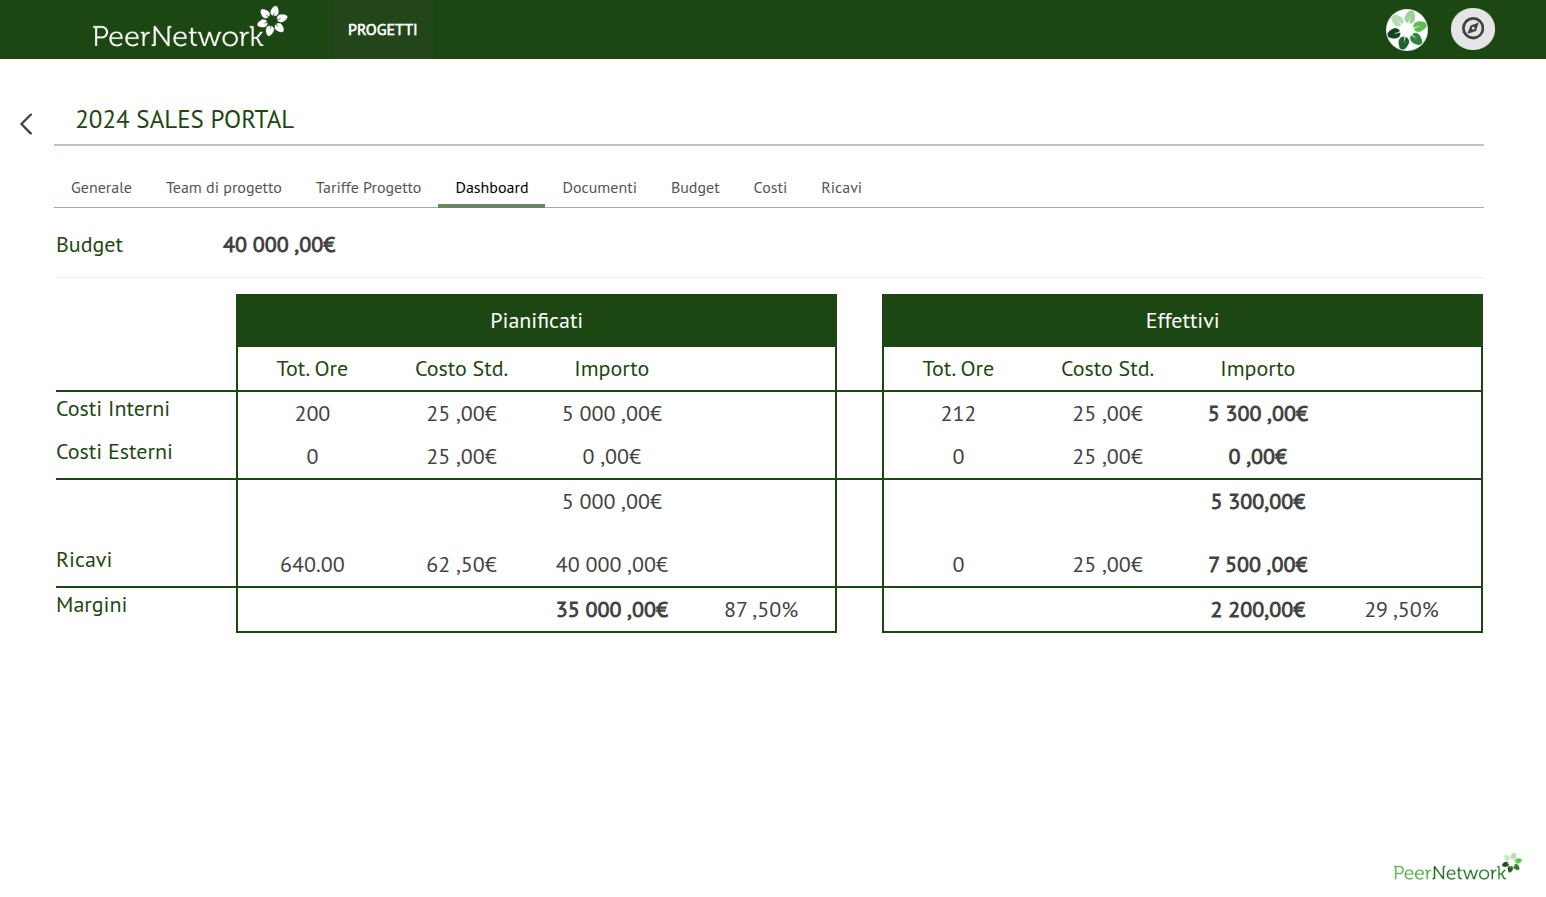
\includegraphics[width=\linewidth]{figures/dashboardPAM.png}
    \caption{Dashboard riepilogativa dei dati economici di un progetto}
    \label{fig:pam-dashboard}
\end{figure}
\section{Peer Network Activity Management}
Nell'area Progetti dell’applicazione \ac{PAM}, ogni progetto gestito dall’azienda dispone di una sezione dedicata
contenente tutte le informazioni rilevanti.
Come mostrato in Figura \ref{fig:pam-dashboard}, i dati specifici del progetto sono organizzati in diverse categorie:
informazioni generali (contenenti ad esempio cliente, budget e scadenze), composizione del team, tariffe di progetto
(costo giornaliero per dipendente in base al ruolo), oltre a riepiloghi economici e documenti (come le pre-fatture emesse).
In particolare, l'immagine riporta l'interfaccia principale sviluppata, attualmente già in uso dalla direzione e
dall'area amministrativa, denominata dashboard. Per motivi di riservatezza, la schermata presenta dati fittizi relativi
a un progetto simulato.

Basandosi sul mockup e sulle funzionalità richieste illustrate nel Capitolo \ref{chap:pam}, l’interfaccia permette
di visualizzare costi, ricavi e margini, sia pianificati che effettivi.
Alcuni valori pianificati, come il budget (indicato anche come importo del ricavo previsto) e le ore considerate
come costo interno, vengono inseriti dal project manager nella sezione riguardo le informazioni generali
del progetto, descritta in precedenza.
Il costo standard, utilizzato per il calcolo dei ricavi, si basa sulle tariffe di progetto, definite manualmente all’inizio del
progetto nella rispettiva sezione.
Gli altri valori previsionali vengono invece determinati attraverso semplici calcoli basati sui dati già disponibili.
I valori reali, invece, si aggiornano automaticamente: i costi effettivi vengono calcolati in base alle ore di lavoro
registrate dai dipendenti su Jira, mentre i ricavi effettivi derivano dalla somma delle pre-fatture emesse mensilmente al cliente.